\documentclass[11pt]{article}
\usepackage[utf8]{inputenc}	% Para caracteres en español
\usepackage{amsmath,amsthm,amsfonts,amssymb,amscd}
\usepackage{multirow,booktabs}
\usepackage[table]{xcolor}
\usepackage{fullpage}
\usepackage{lastpage}
\usepackage{enumitem}
\usepackage{fancyhdr}
\usepackage{mathrsfs}
\usepackage{wrapfig}
\usepackage{setspace}
\usepackage{calc}
\usepackage{multicol}
\usepackage{cancel}
\usepackage[retainorgcmds]{IEEEtrantools}
\usepackage[margin=1cm]{geometry}
\usepackage{amsmath}
\newlength{\tabcont}
\setlength{\parindent}{0.0in}
\setlength{\parskip}{0.05in}
\usepackage{empheq}
\usepackage{framed}
\usepackage[most]{tcolorbox}
\usepackage{xcolor}
\usepackage{graphicx}
\usepackage{listings}
% -- Basic formatting
\usepackage[utf8]{inputenc}
\usepackage[english]{babel}
\usepackage{times}
\usepackage{caption}
\usepackage{subcaption}
\usepackage{placeins}
\setlength{\parindent}{0pt}
\usepackage{indentfirst}% -- Defining colors:
\usepackage[dvipsnames]{xcolor}
\definecolor{codegreen}{rgb}{0,0.6,0}
\definecolor{codegray}{rgb}{0.5,0.5,0.5}
\definecolor{codepurple}{rgb}{0.58,0,0.82}
\definecolor{backcolour}{rgb}{0.95,0.95,0.92}% Definig a custom style:
\lstdefinestyle{mystyle}{
    backgroundcolor=\color{backcolour},   
    commentstyle=\color{codepurple},
    keywordstyle=\color{NavyBlue},
    numberstyle=\tiny\color{codegray},
    stringstyle=\color{codepurple},
    basicstyle=\ttfamily\footnotesize\bfseries,
    breakatwhitespace=false,         
    breaklines=true,                 
    captionpos=t,                    
    keepspaces=true,                 
    numbers=left,                    
    numbersep=5pt,                  
    showspaces=false,                
    showstringspaces=false,
    showtabs=false,                  
    tabsize=2
}% -- Setting up the custom style:
\lstset{style=mystyle}
\lstset{
  style=mystyle,
  framexleftmargin=3.5mm,
  rulesepcolor=\color{black},
  linewidth=0.6\linewidth,
  xleftmargin=12pt,
  aboveskip=12pt,
  belowskip=12pt
}
\colorlet{shadecolor}{orange!15}
\parindent 0in
\parskip 1pt
\geometry{margin=1in, headsep=0.25in}
\theoremstyle{definition}
\newtheorem{defn}{Definition}
\newtheorem{reg}{Rule}
\newtheorem{exer}{Exercise}
\newtheorem{note}{Note}
\graphicspath{ {./images/} }
\begin{document}
\setcounter{section}{0}
\title{MIE223 Lecture Notes}

\thispagestyle{empty}

\begin{center}
{\LARGE \bf Time Series Data}\\
{\large MIE223}\\
Winter 2025
\end{center}
\section{Time Series Analysis}
\subsection{Time Series Data}
\begin{itemize}
  \item Time series data are
  \item Observations or measurements that
  are indexed according to time
  \item Instead of Xi we have Xt where t is
  specifically a time index
  \item Why does time make it different?
  \item The time index t has a special ordering
  \item Data measured over time are not
  exchangeable, which is what we often
  assume when data are indexed by i
\end{itemize}
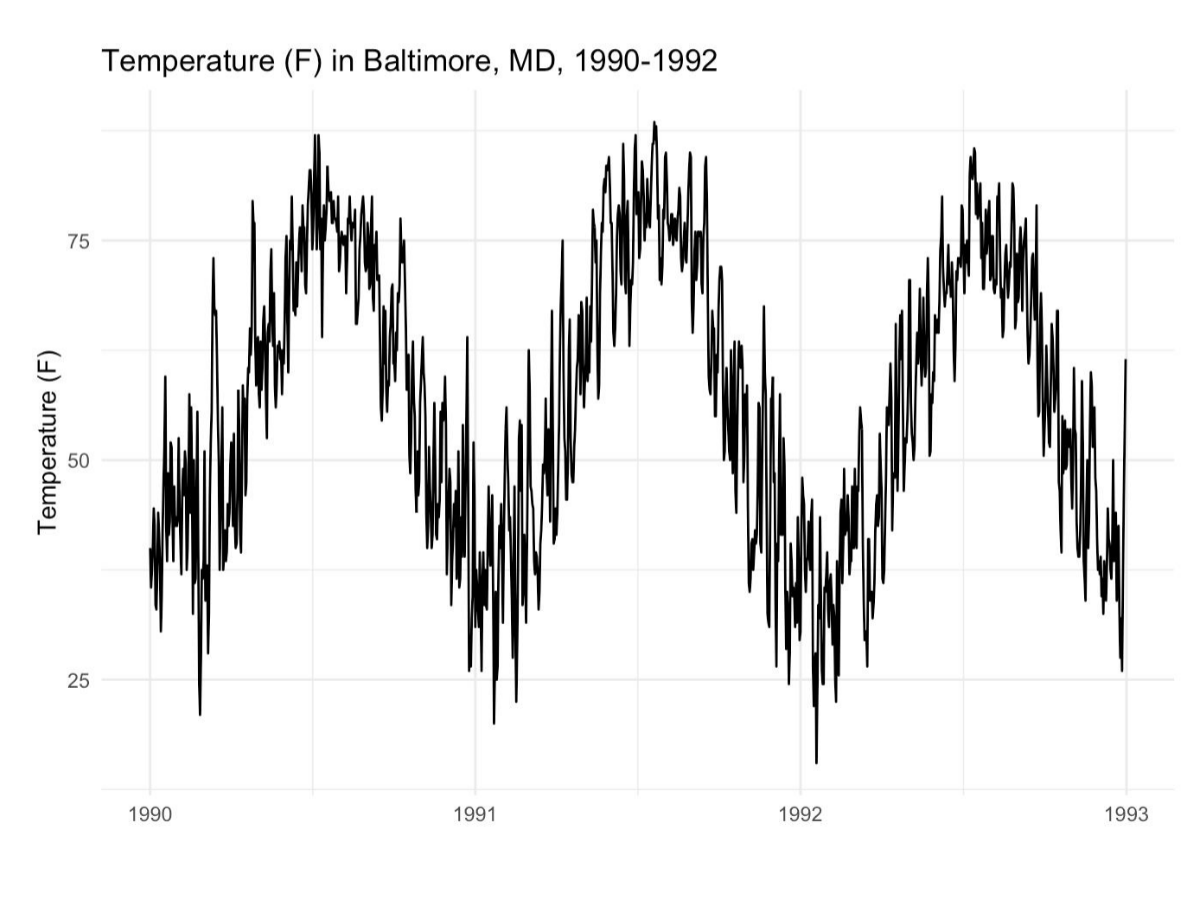
\includegraphics[width=\textwidth]{1.png}

\subsection{Goals of Time Series Analysis}
\begin{itemize}
  \item Time Scale Analysis: at what scale is data useful to analyze?
  \item Is weather useful to analyze at the second, hour, or year level? Is it seasonal?
  \item Smoothing: infer true state of past given a noisy signal (averaging out nearby timepoints)
  \item Assuming gradual change, use nearby values in a time series to smooth noise
  \item Filtering: what is the true present state given a noisy signal
  \item Tracking a rocket trajectory
  \item Kalman filtering!
  \item Forecasting: predict future values
  \item What will the stock price be tomorrow, given the past?
  \item Regression: give time two series, can we predict the association between them?
  \item Does public sentiment predict the stock market at a delay?
\end{itemize}

\section{Time Scale Analysis}
\subsection{Time Scale Analysis}
\begin{itemize}
  \item What time scales of variation dominate or account for the
  majority of temporal variation in the data? seasonal
  \item Is there a strong seasonal cycle in the observations of
  temperature in Baltimore, MD? Hope so
  \item Is the association between ambient air pollution and mortality in
  a city primarily driven by large annual changes in pollution
  levels or by short-term spikes? there can be multiple causes of mortality, and need longer timeframe
  \item granger causality says that you can predict something if you know the past
\end{itemize}

\subsection{Trend-Season-Residual Decomposition}
A common tool to use is to
decompose a time series into

\begin{enumerate}
  \item Smooth long-term trend (trend)
  \item Seasonal variation (seasonal)
  \item Residual variation (day to day)
\end{enumerate}

The primary benefit is of
looking at long-term trend
and seasonal variation is that
they are highly interpretable
and are very common.

These graphs can be made by smoothing over different intervals.

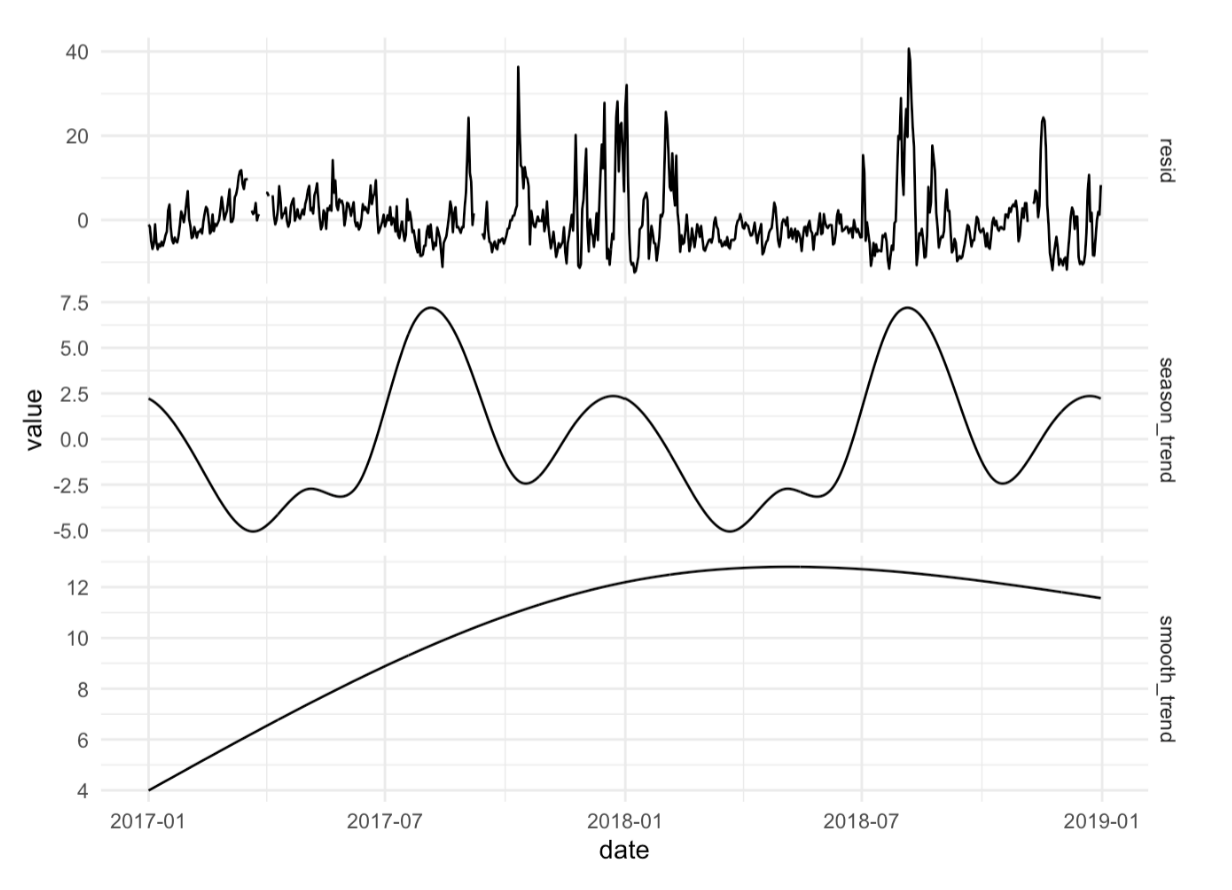
\includegraphics[width=\textwidth]{2.png}

\subsection{Trend-Season-Residual Example 1}
\begin{itemize}
  \item Daily and monthly
  temperature vs. year
  • What time scales are
  informative?
  \item What do you think
  could be
  \begin{itemize}
    \item Long-term trend: climate change
    \item Is there seasonality? weather seasons
    \item Cause of variation? day to day fluctuations in the weather
  \end{itemize}
\end{itemize}

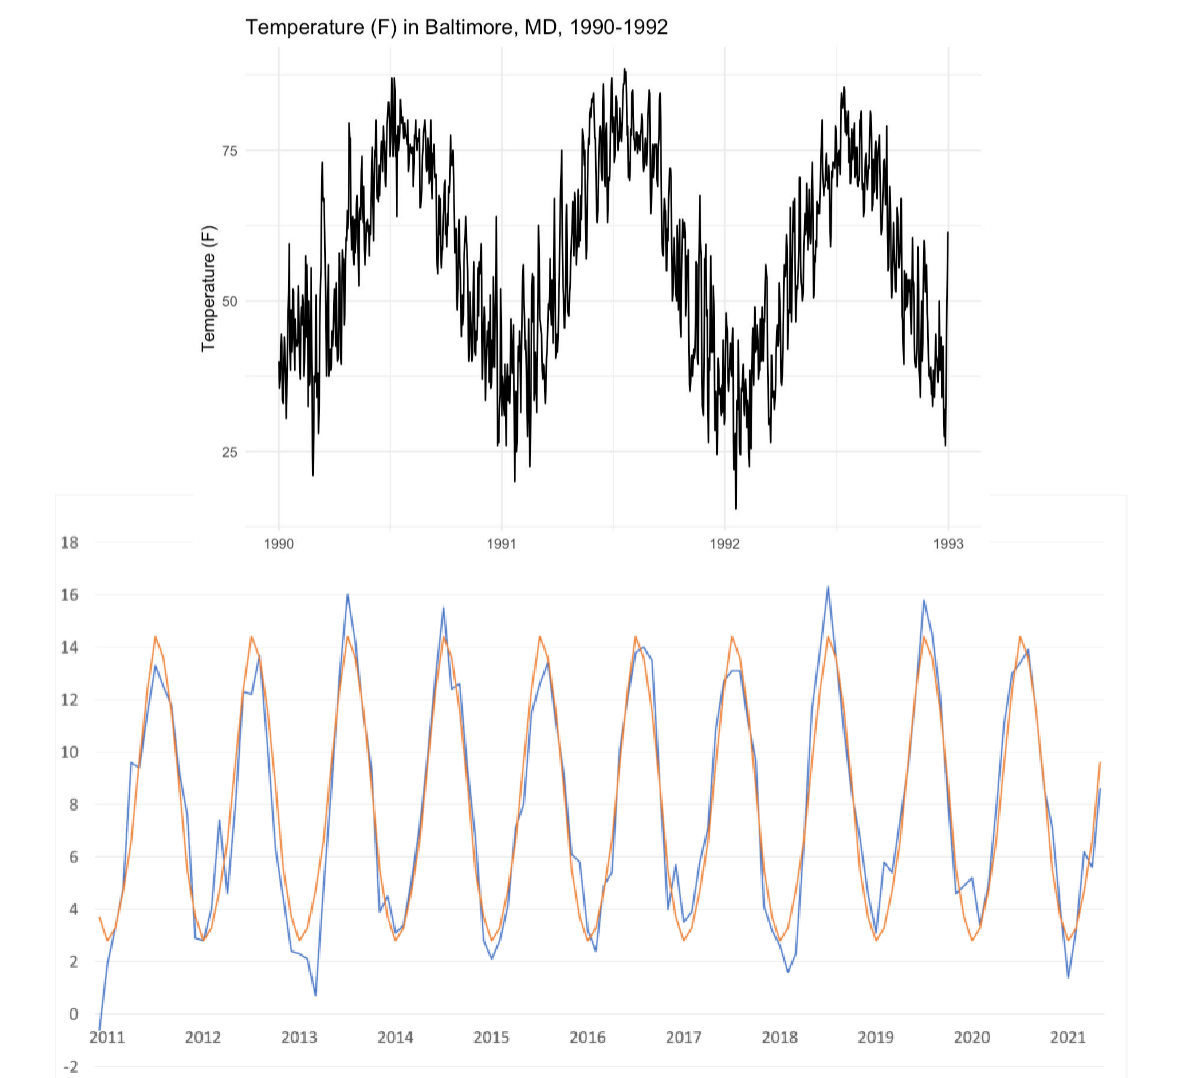
\includegraphics[width=\textwidth]{3.png}

\subsection{Trend-Season-Residual Example 2}
Three stocks: GOOG,
MSFT, ZOOM
• Which is which?

\begin{itemize}
  \item What do you think
  could be
  \begin{itemize}
    \item Long-term trend
    \item Is there seasonality?
    \item Cause of variation?
  \end{itemize}
\end{itemize}

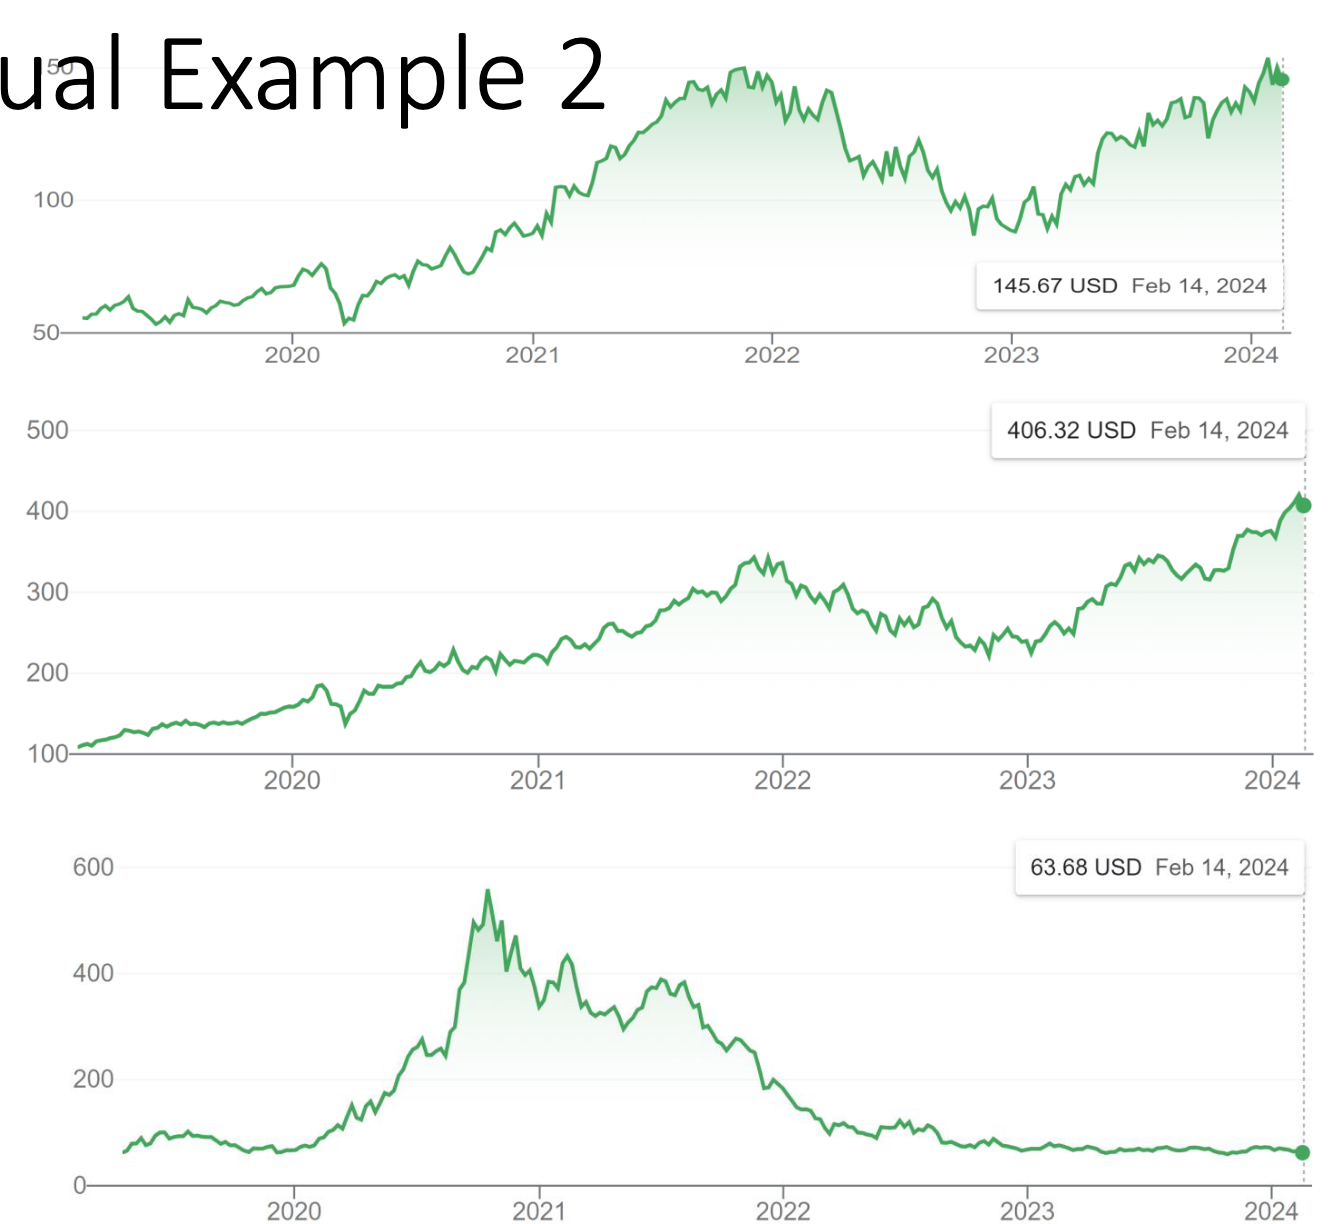
\includegraphics[width=\textwidth/4]{4.png}

\section{Time Series Regression with
Autocorrelation and
Cross-correlation}
\subsection{Regression (in general)}
Given a time series of two phenomena, what is the association
between them?

\begin{itemize}
  \item What is the association between daily levels of air pollution and daily
  values of cardiac hospitalizations?
  \item What is the lag (in months) between a change in a country’s
  unemployment rate and a change in the gross domestic product?
  \item What is the cumulative number of excess deaths that occurs in the 2
  weeks following a major hurricane?
\end{itemize}

\subsection{Recap of Covariance}
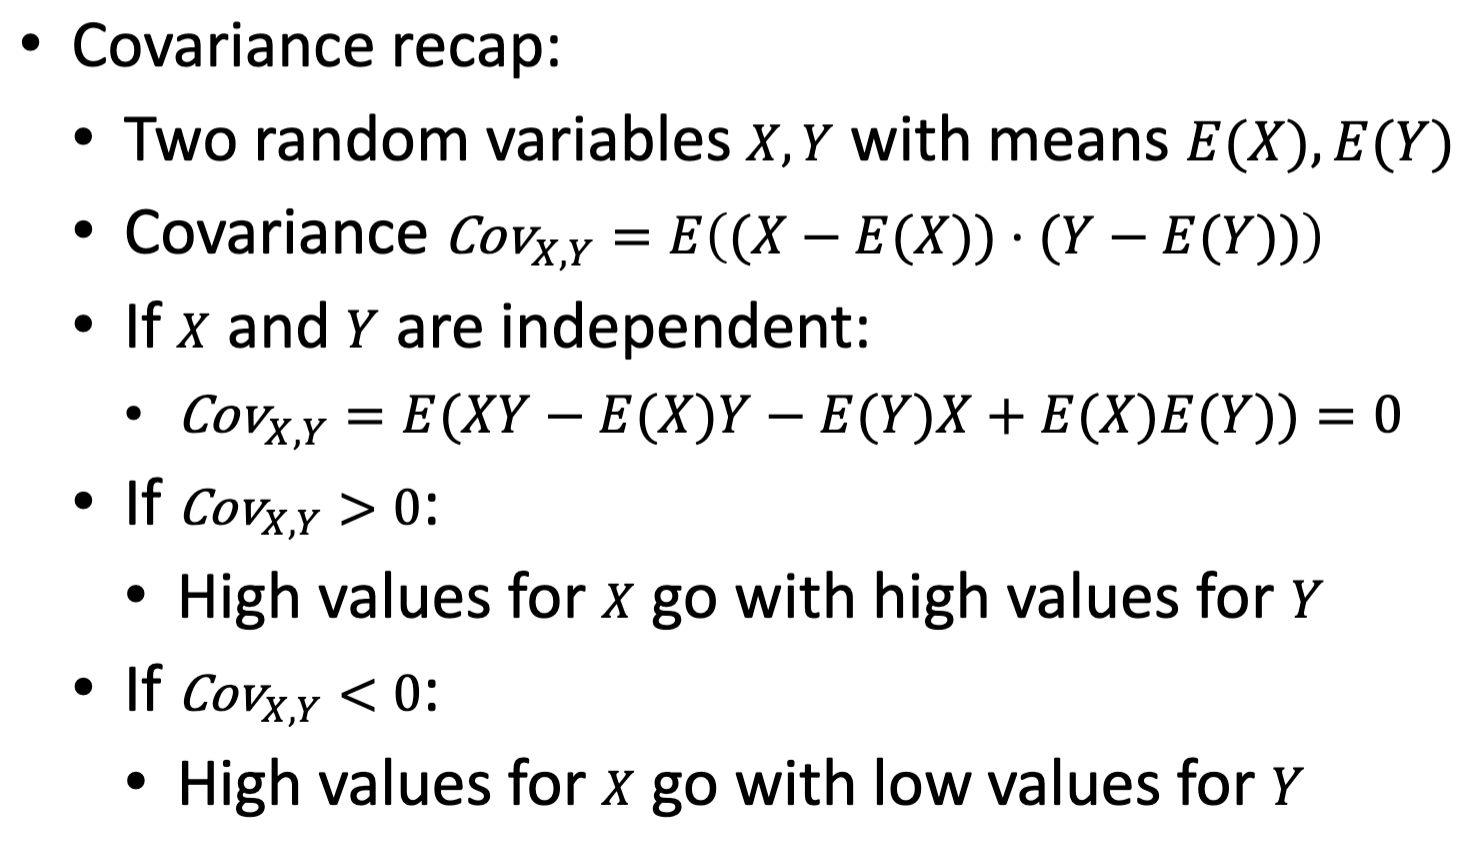
\includegraphics[width=\textwidth/2]{5.png}

\subsection{Pearson Correlation Coefficient}
Covariance depends on the units in which X and Y are given

Therefore, we look at the Pearson correlation coefficient

If x and y have standard deviations $\sigma x$ and $\sigma y$ respectively:

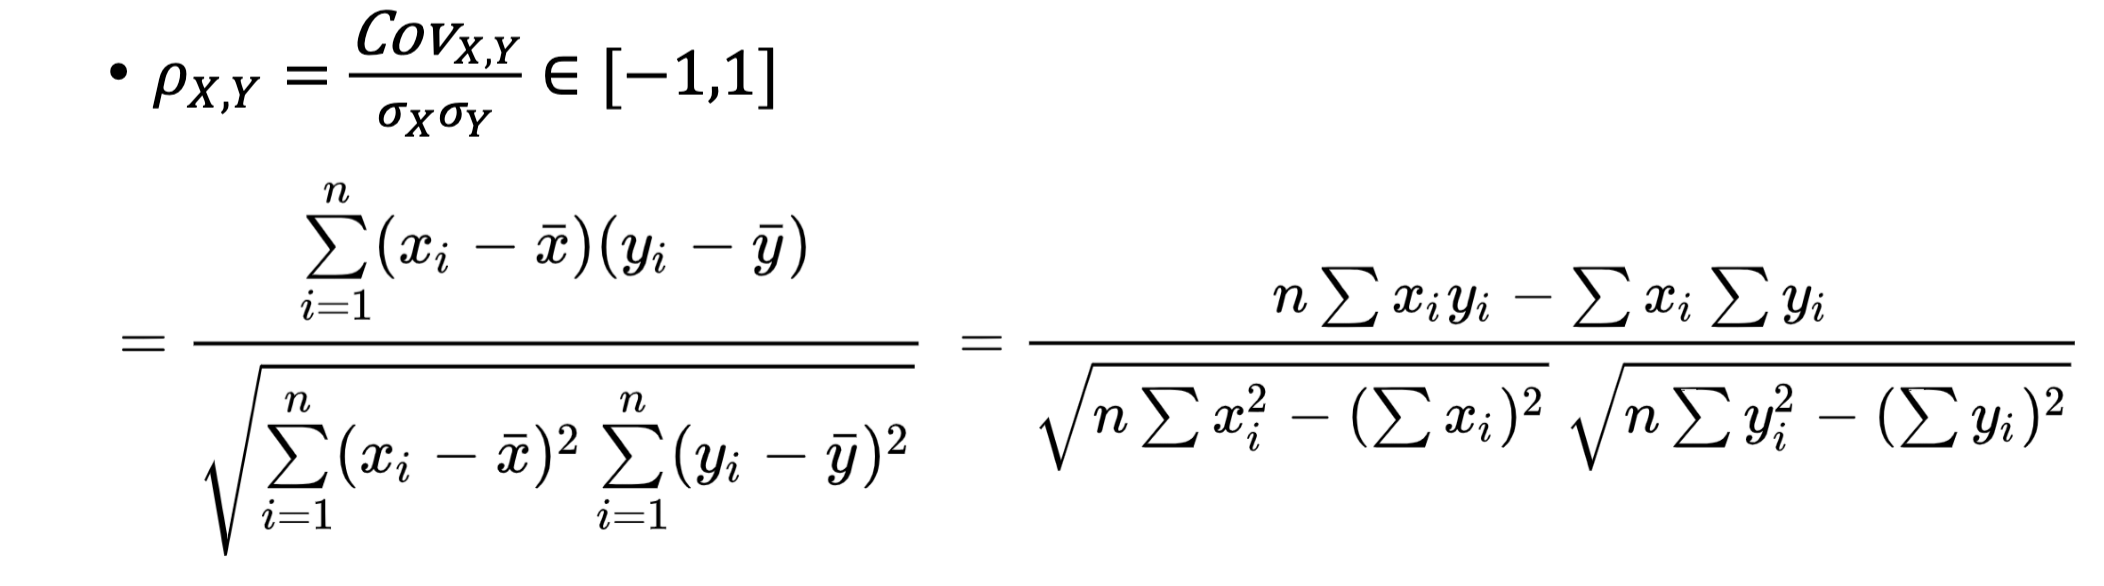
\includegraphics[width=\textwidth/2]{6.png}

\subsection{Autocorrelation}
Auto-correlation: Compare the correlation of a time series with itself
moved (lagged) by k positions

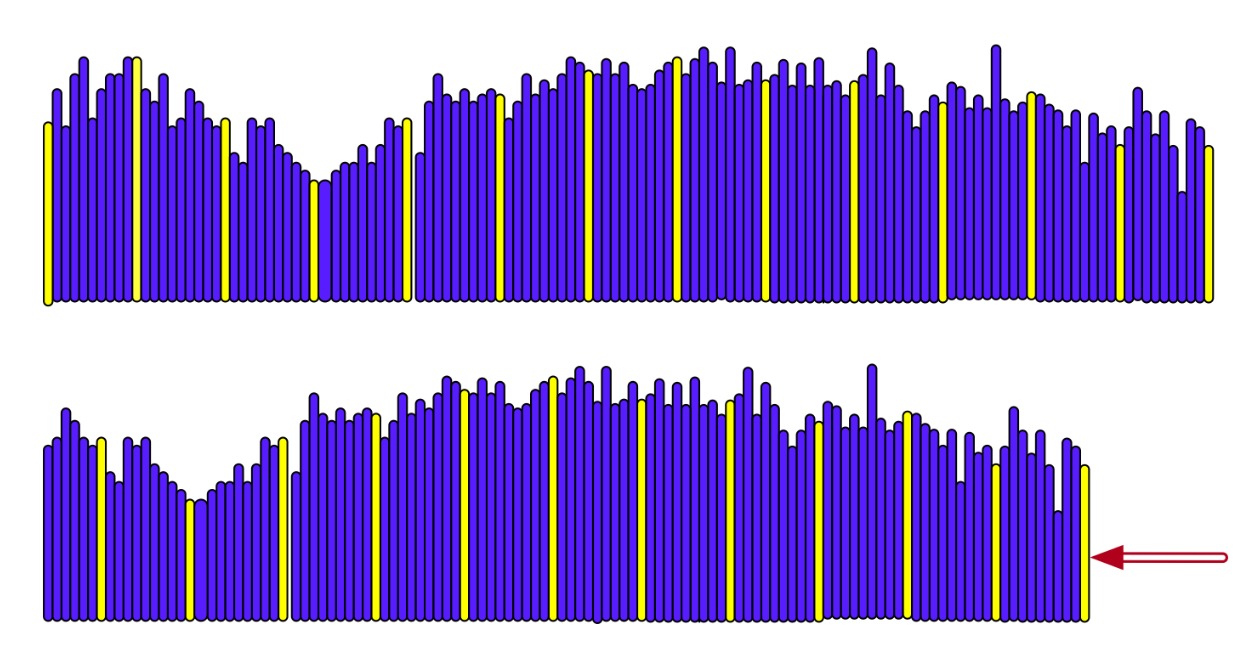
\includegraphics[width=\textwidth/2]{7.png}

\subsection{Autocorrelation:
Measure of correlation in time series
at different lags}
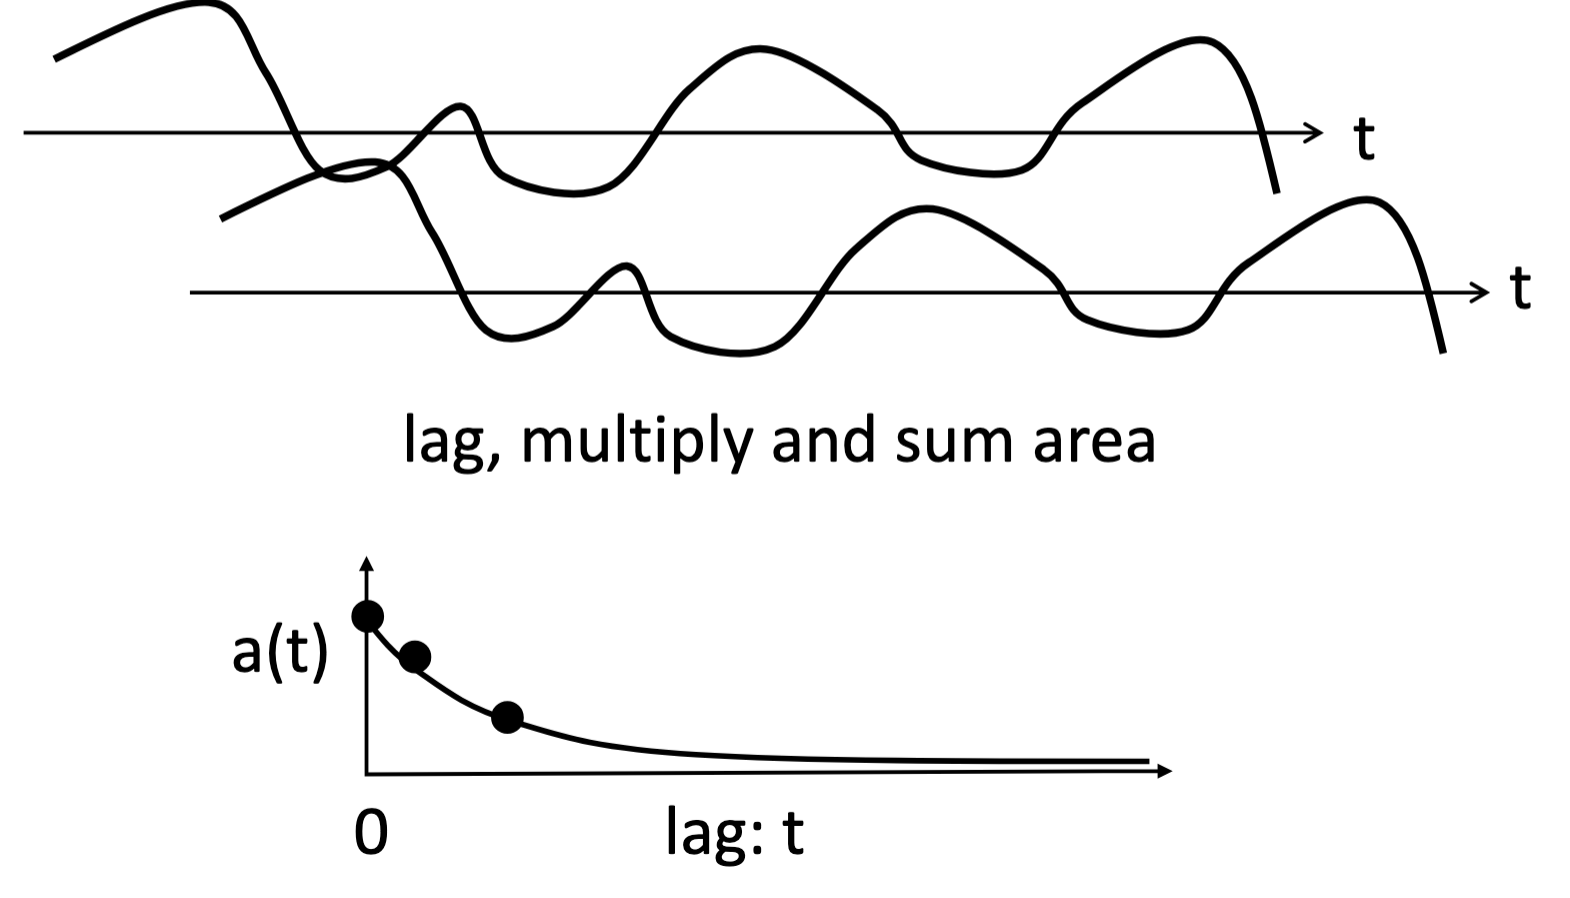
\includegraphics[width=\textwidth/2]{8.png}

\subsection{Autocorrelation Example}
Autocorrelation for
Chenai temperatures

\begin{itemize}
  \item High auto-correlation
  for the next day and
  for a year afterwards
  \item The light blue
  denotes significance
\end{itemize}

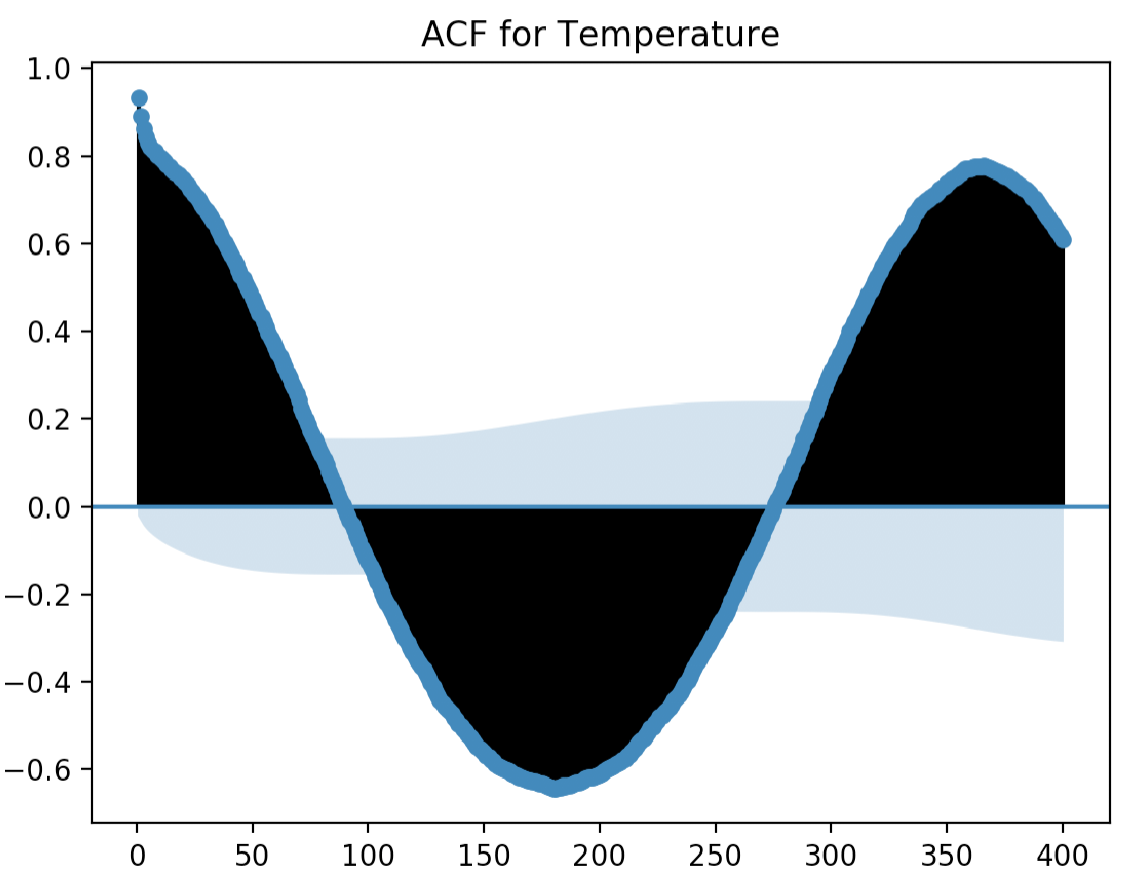
\includegraphics[width=\textwidth/2]{9.png}

\subsection{Cross-correlation}
\begin{itemize}
  \item Consider how one time
  series “predicts another”
  \begin{itemize}
    \item Example: how does the
    amount of rainfall affect
    (predict) the discharge water
    flow rate of a river measured
    at a given point?
    \begin{itemize}
      \item Discharge correlated with rain
      \item Discharge is delayed behind
      rain because rain takes time
      to drain from the land
    \end{itemize}
  \end{itemize}
\end{itemize}

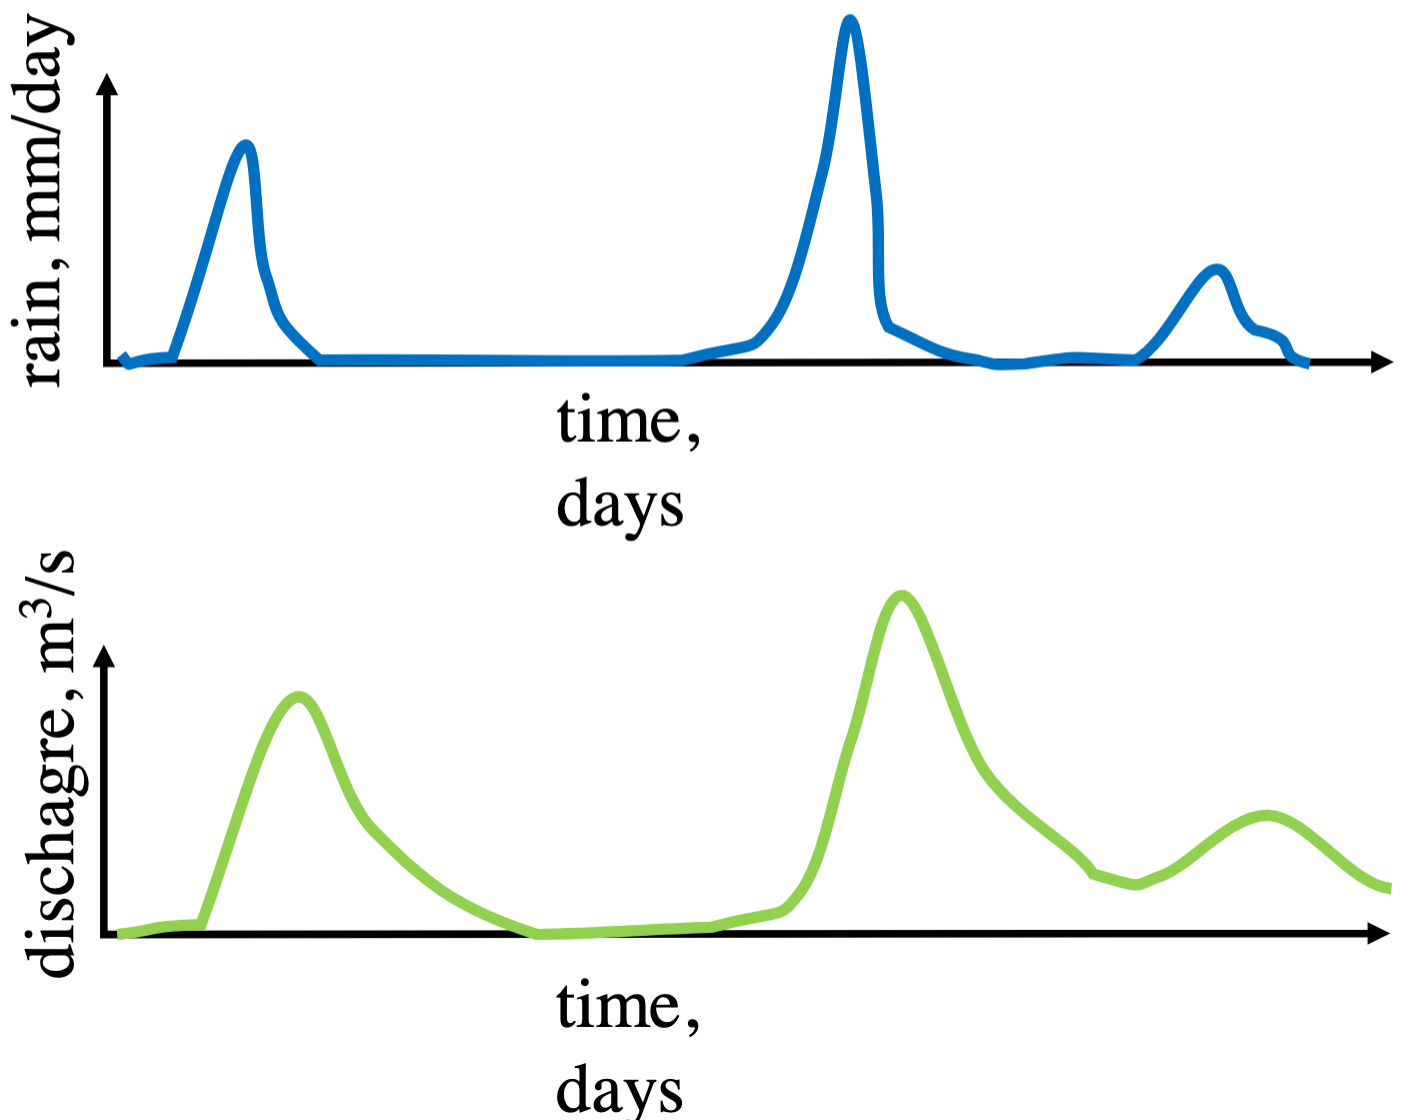
\includegraphics[width=\textwidth/2]{10.png}

Sample midterm question: Would you use VADER to predict the stock market?

Answer: No, VADER is a sentiment analysis tool that is used to analyze text data. It is not used to predict the stock market.
Simple polarity sentiment is not complex enough to analyze the stock market

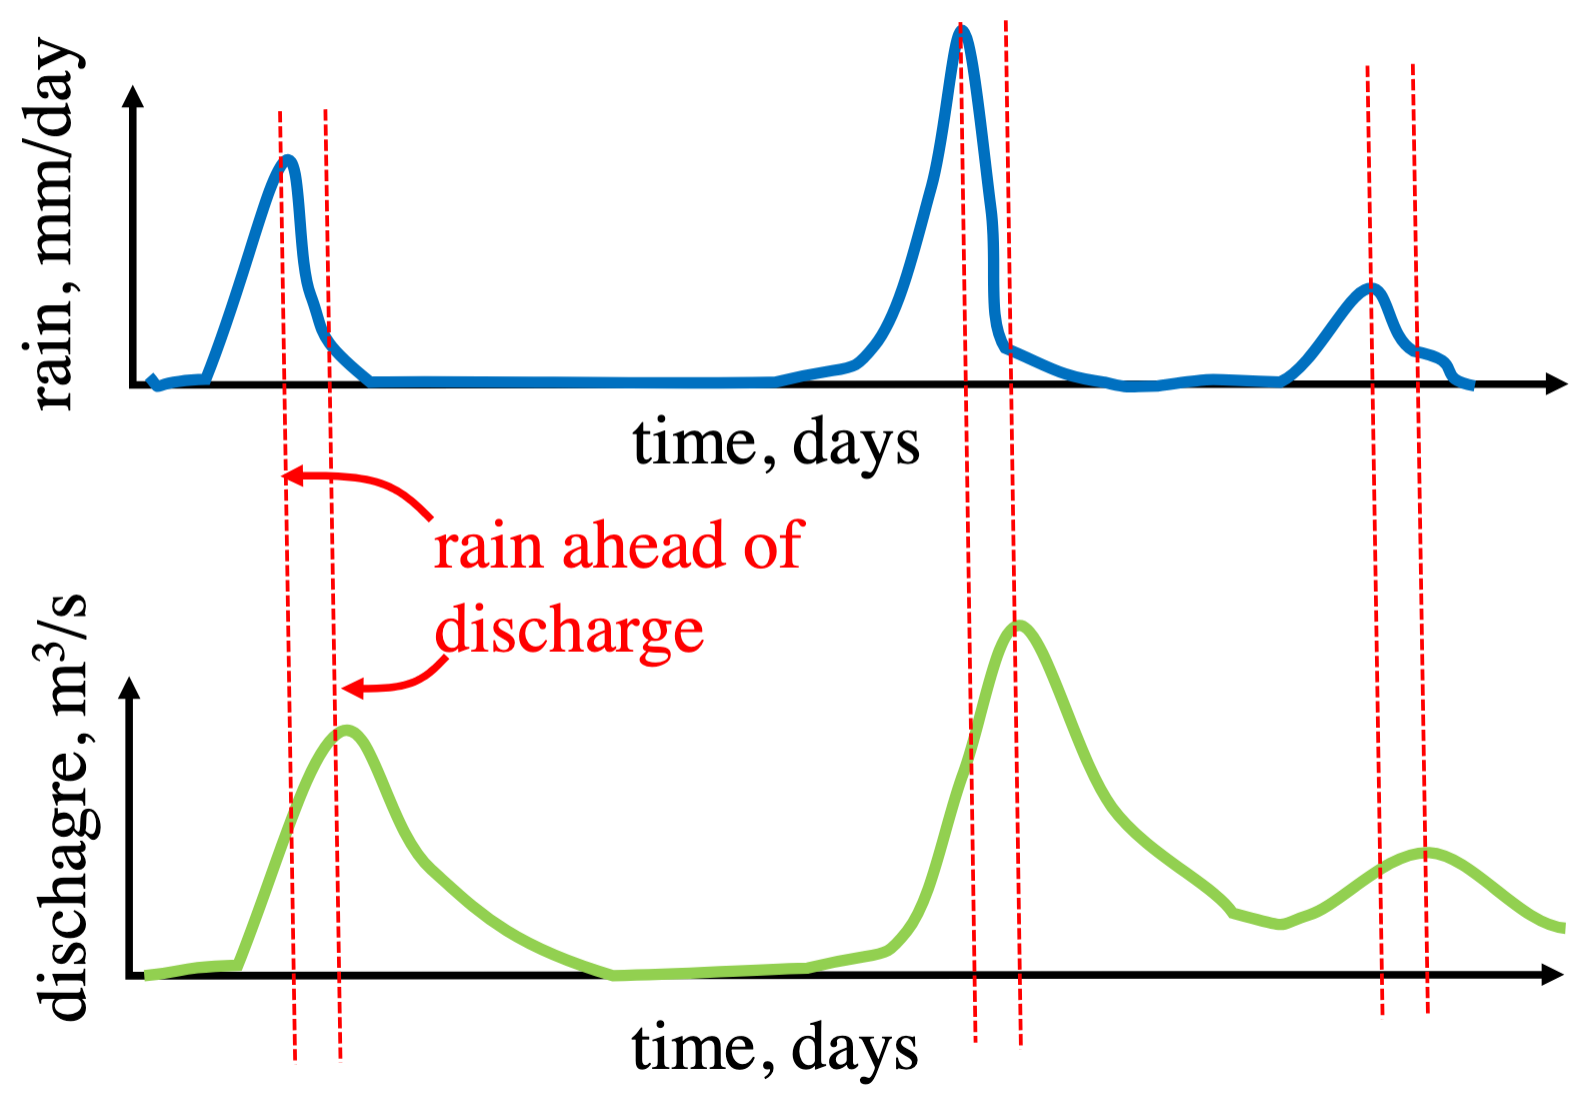
\includegraphics[width=\textwidth/4]{11.png}
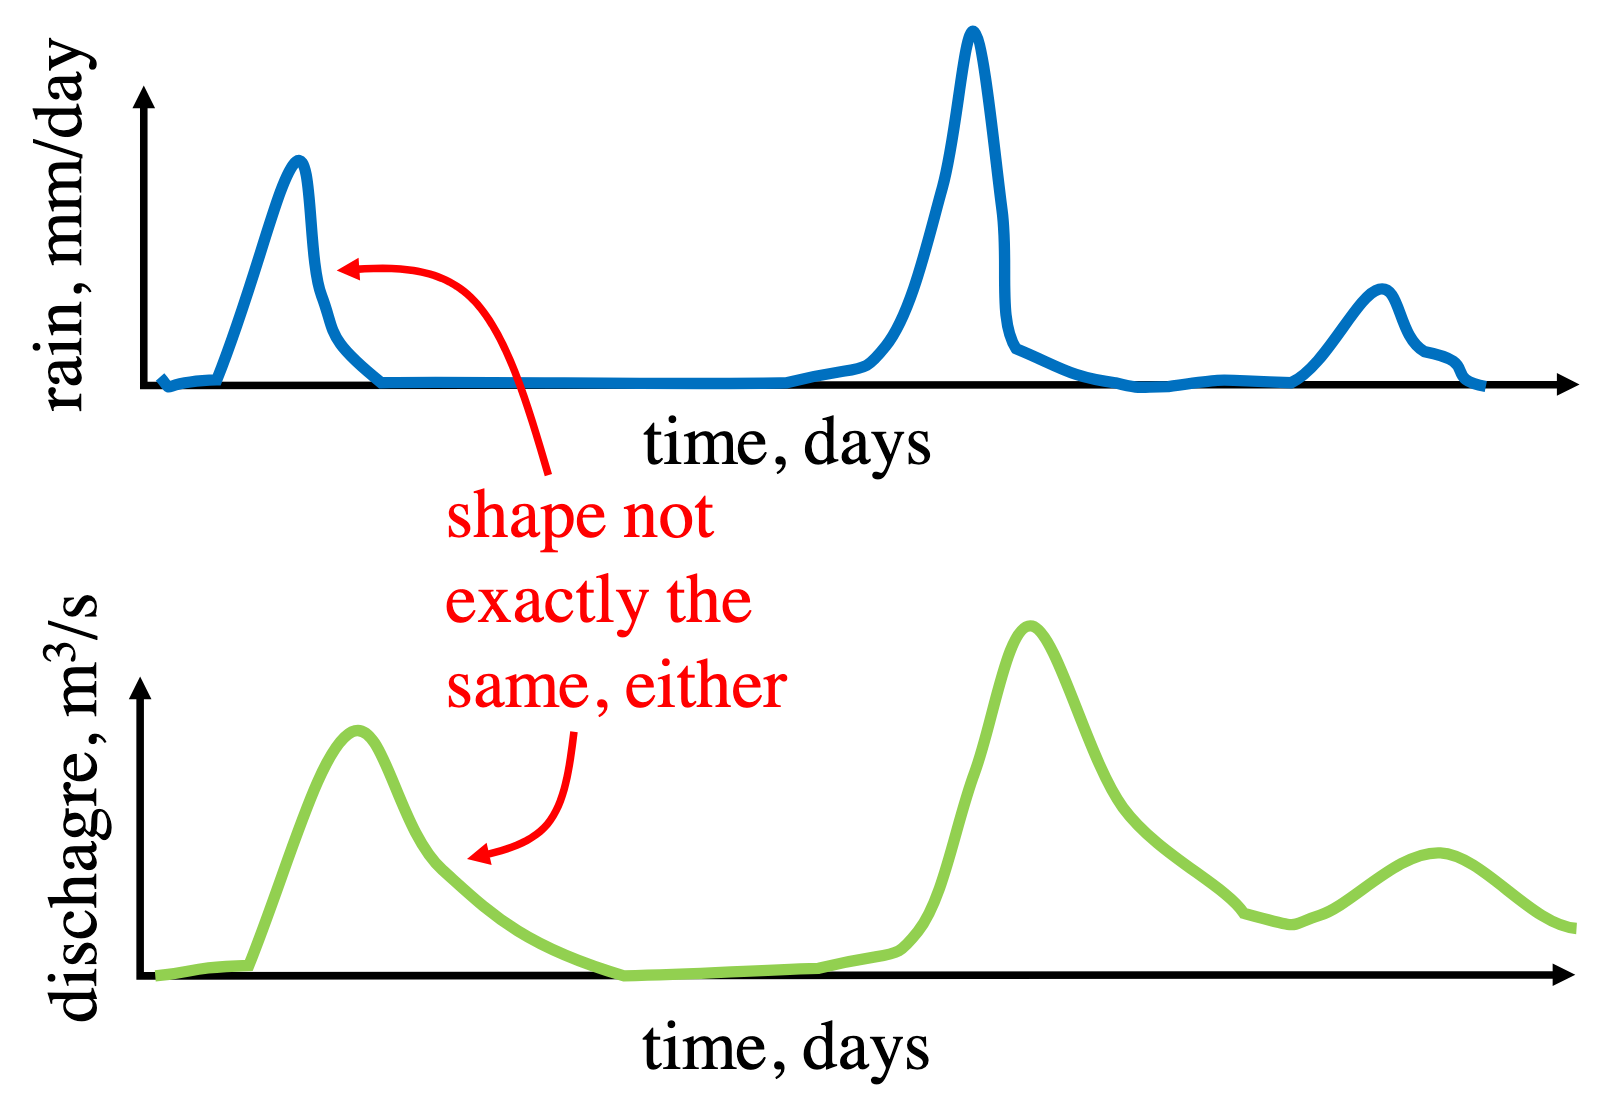
\includegraphics[width=\textwidth/4]{12.png}

\subsection{Cross-correlation
Measure of correlation between two time series
at different lags}

\includegraphics[width=\textwidth/2]{13.png}

\section{Smoothing}


\end{document}